%%%% For double-blind review submission, w/o CCS and ACM Reference (max submission space)
\documentclass[10pt, sigplan]{acmart}
%%\settopmatter{printfolios=true,printccs=false,printacmref=false}
%% For double-blind review submission, w/ CCS and ACM Reference
%\documentclass[sigplan,10pt,review,anonymous]{acmart}\settopmatter{printfolios=true}
%% For single-blind review submission, w/o CCS and ACM Reference (max submission space)
%\documentclass[sigplan,10pt,review]{acmart}\settopmatter{printfolios=true,printccs=false,printacmref=false}
%% For single-blind review submission, w/ CCS and ACM Reference
%\documentclass[sigplan,10pt,review]{acmart}\settopmatter{printfolios=true}
%% For final camera-ready submission, w/ required CCS and ACM Reference
%\documentclass[sigplan,10pt]{acmart}\settopmatter{}


%% Conference information
%% Supplied to authors by publisher for camera-ready submission;
%% use defaults for review submission.
%\acmConference[PL'17]{ACM SIGPLAN Conference on Programming Languages}{January 01--03, 2017}{New York, NY, USA}
%\acmYear{2017}
%\acmISBN{} % \acmISBN{978-x-xxxx-xxxx-x/YY/MM}
%\acmDOI{} % \acmDOI{10.1145/nnnnnnn.nnnnnnn}
%\startPage{1}

%% Copyright information
%% Supplied to authors (based on authors' rights management selection;
%% see authors.acm.org) by publisher for camera-ready submission;
%% use 'none' for review submission.
\setcopyright{none}
%\setcopyright{acmcopyright}
%\setcopyright{acmlicensed}
%\setcopyright{rightsretained}
%\copyrightyear{2017}           %% If different from \acmYear

%% Bibliography style

%\bibliographystyle{ACM-Reference-Format}

%% Citation style
%\citestyle{acmauthoryear}  %% For author/year citations
\citestyle{acmnumeric}     %% For numeric citations
%\setcitestyle{nosort}      %% With 'acmnumeric', to disable automatic
                            %% sorting of references within a single citation;
                            %% e.g., \cite{Smith99,Carpenter05,Baker12}
                            %% rendered as [14,5,2] rather than [2,5,14].
%\setcitesyle{nocompress}   %% With 'acmnumeric', to disable automatic
                            %% compression of sequential references within a
                            %% single citation;
                            %% e.g., \cite{Baker12,Baker14,Baker16}
                            %% rendered as [2,3,4] rather than [2-4].


%%%%%%%%%%%%%%%%%%%%%%%%%%%%%%%%%%%%%%%%%%%%%%%%%%%%%%%%%%%%%%%%%%%%%%
%% Note: Authors migrating a paper from traditional SIGPLAN
%% proceedings format to PACMPL format must update the
%% '\documentclass' and topmatter commands above; see
%% 'acmart-pacmpl-template.tex'.
%%%%%%%%%%%%%%%%%%%%%%%%%%%%%%%%%%%%%%%%%%%%%%%%%%%%%%%%%%%%%%%%%%%%%%


%% Some recommended packages.
\usepackage{booktabs}   %% For formal tables:
                        %% http://ctan.org/pkg/booktabs
\usepackage{subcaption} %% For complex figures with subfigures/subcaptions
                        %% http://ctan.org/pkg/subcaption
\usepackage{xspace}
\usepackage{graphicx}
\usepackage{ifthen}
\usepackage{pgfplots}
\usepackage{listings}
\usepackage{multirow}
\usepgfplotslibrary{statistics}
\usepackage{dblfloatfix} %enable fig at bottom of page
%



% Source Code
%\usepackage{color}
%\usepackage{textcomp}
%\usepackage{listings}
%\usepackage{ulem}
%\usepackage[T1]{fontenc}
%\usepackage{times}
% \usepackage{needspace}
 

% Source Code
\usepackage{color}
\usepackage{textcomp}
\usepackage{listings}

\definecolor{source}{gray}{0.85}% my comment style
\newcommand{\myCommentStyle}[1]{{\footnotesize\sffamily\color{gray!100!white} #1}}
%\newcommand{\myCommentStyle}[1]{{\footnotesize\sffamily\color{black!100!white} #1}}

% my string style
\newcommand{\myStringStyle}[1]{{\footnotesize\sffamily\color{violet!100!black} #1}}
%\newcommand{\myStringStyle}[1]{{\footnotesize\sffamily\color{black!100!black} #1}}

% my symbol style
\newcommand{\mySymbolStyle}[1]{{\footnotesize\sffamily\color{violet!100!black} #1}}
%\newcommand{\mySymbolStyle}[1]{{\footnotesize\sffamily\color{black!100!black} #1}}

% my keyword style
\newcommand{\myKeywordStyle}[1]{{\footnotesize\sffamily\color{green!70!black} #1}}
%\newcommand{\myKeywordStyle}[1]{{\footnotesize\sffamily\color{black!70!black} #1}}

% my global style
\newcommand{\myGlobalStyle}[1]{{\footnotesize\sffamily\color{blue!100!black} #1}}
%\newcommand{\myGlobalStyle}[1]{{\footnotesize\sffamily\color{black!100!black} #1}}

% my number style
\newcommand{\myNumberStyle}[1]{{\footnotesize\sffamily\color{brown!100!black} #1}}
%\newcommand{\myNumberStyle}[1]{{\footnotesize\sffamily\color{black!100!black} #1}}

\lstset{
language={},
% characters
tabsize=3,
escapechar={!},
keepspaces=true,
breaklines=true,
alsoletter={\#},
literate={\$}{{{\$}}}1,
breakautoindent=true,
columns=fullflexible,
showstringspaces=false,
% background
frame=single,
aboveskip=1em, % automatic space before
framerule=0pt,
basicstyle=\footnotesize\sffamily\color{black},
keywordstyle=\myKeywordStyle,% keyword style
commentstyle=\myCommentStyle,% comment style
frame=single,%
backgroundcolor=\color{source},
% numbering
stepnumber=1,
numbersep=10pt,
numberstyle=\tiny,
numberfirstline=true,
% caption
captionpos=b,
% formatting (html)
moredelim=[is][\bfseries]{<b>}{</b>},
moredelim=[is][\textit]{<i>}{</i>},
moredelim=[is][\underbar]{<u>}{</u>},
moredelim=[is][\color{red}\uwave]{<wave>}{</wave>},
moredelim=[is][\color{red}\sout]{<del>}{</del>},
moredelim=[is][\color{blue}\underbar]{<ins>}{</ins>},
% smalltalk stuff
morecomment=[s][\myCommentStyle]{"}{"},
%    morecomment=[s][\myvs]{|}{|},
morestring=[b][\myStringStyle]',
moredelim=[is][]{<sel>}{</sel>},
moredelim=[is][]{<rcv>}{</rcv>},
moredelim=[is][\itshape]{<symb>}{</symb>},
moredelim=[is][\scshape]{<class>}{</class>},
morekeywords={true,false,nil,self,super,thisContext},
identifierstyle=\idstyle,
}

\makeatletter
\newcommand*\idstyle[1]{%
\expandafter\id@style\the\lst@token{#1}\relax%
}
\def\id@style#1#2\relax{%
\ifnum\pdfstrcmp{#1}{\#}=0%
% this is a symbol
\mySymbolStyle{\the\lst@token}%
\else%
\edef\tempa{\uccode`#1}%
\edef\tempb{`#1}%
\ifnum\tempa=\tempb%
% this is a global
\myGlobalStyle{\the\lst@token}%
\else%
\the\lst@token%
\fi%
\fi%
}
\makeatother


%\newcommand{\ct}{\lstinline[backgroundcolor=\color{white}]}
%\newcommand{\needlines}[1]{\Needspace{#1\baselineskip}}
\newcommand{\lct}{\texttt}

\lstnewenvironment{code}{%
    \lstset{%
    % frame=lines,
    frame=single,
    framerule=0pt,
    mathescape=false
    }%
    \noindent%
    \minipage{\linewidth}%
}{%
    \endminipage%
}%


\lstnewenvironment{codeWithLineNumbers}{%
    \lstset{%
    % frame=lines,
    frame=single,
    framerule=0pt,
    mathescape=false,
    numbers=left
    }%
    \noindent%
    \minipage{\linewidth}%
}{%
    \endminipage%
}%



\newenvironment{codeNonSmalltalk}
{\begin{alltt}\sffamily}
{\end{alltt}\normalsize}



\usepackage{xcolor}
\newcommand{\todo}[1]{\color{orange}\fbox{\bfseries\sffamily\scriptsize TODO:}{\sf\small$\blacktriangleright$\textit{#1}$\blacktriangleleft$}\color{black}}
\newcommand{\sk}[1]{\color{blue}\fbox{\bfseries\sffamily\scriptsize Sophie:}{\sf\small$\blacktriangleright$\textit{#1}$\blacktriangleleft$}\color{black}}
\newcommand{\cba}[1]{\color{purple}\fbox{\bfseries\sffamily\scriptsize Clement:}{\sf\small$\blacktriangleright$\textit{#1}$\blacktriangleleft$}\color{black}}
%\newcommand*{rotatebox{75}}




% Source Code
%\usepackage{color}
%\usepackage{textcomp}
%\usepackage{listings}
%\usepackage{ulem}
%\usepackage[T1]{fontenc}
%\usepackage{times}
% \usepackage{needspace}
 

% Source Code
\usepackage{color}
\usepackage{textcomp}
\usepackage{listings}

\definecolor{source}{gray}{0.85}% my comment style
\newcommand{\myCommentStyle}[1]{{\footnotesize\sffamily\color{gray!100!white} #1}}
%\newcommand{\myCommentStyle}[1]{{\footnotesize\sffamily\color{black!100!white} #1}}

% my string style
\newcommand{\myStringStyle}[1]{{\footnotesize\sffamily\color{violet!100!black} #1}}
%\newcommand{\myStringStyle}[1]{{\footnotesize\sffamily\color{black!100!black} #1}}

% my symbol style
\newcommand{\mySymbolStyle}[1]{{\footnotesize\sffamily\color{violet!100!black} #1}}
%\newcommand{\mySymbolStyle}[1]{{\footnotesize\sffamily\color{black!100!black} #1}}

% my keyword style
\newcommand{\myKeywordStyle}[1]{{\footnotesize\sffamily\color{green!70!black} #1}}
%\newcommand{\myKeywordStyle}[1]{{\footnotesize\sffamily\color{black!70!black} #1}}

% my global style
\newcommand{\myGlobalStyle}[1]{{\footnotesize\sffamily\color{blue!100!black} #1}}
%\newcommand{\myGlobalStyle}[1]{{\footnotesize\sffamily\color{black!100!black} #1}}

% my number style
\newcommand{\myNumberStyle}[1]{{\footnotesize\sffamily\color{brown!100!black} #1}}
%\newcommand{\myNumberStyle}[1]{{\footnotesize\sffamily\color{black!100!black} #1}}

\lstset{
language={},
% characters
tabsize=3,
escapechar={!},
keepspaces=true,
breaklines=true,
alsoletter={\#},
literate={\$}{{{\$}}}1,
breakautoindent=true,
columns=fullflexible,
showstringspaces=false,
% background
frame=single,
aboveskip=1em, % automatic space before
framerule=0pt,
basicstyle=\footnotesize\sffamily\color{black},
keywordstyle=\myKeywordStyle,% keyword style
commentstyle=\myCommentStyle,% comment style
frame=single,%
backgroundcolor=\color{source},
% numbering
stepnumber=1,
numbersep=10pt,
numberstyle=\tiny,
numberfirstline=true,
% caption
captionpos=b,
% formatting (html)
moredelim=[is][\bfseries]{<b>}{</b>},
moredelim=[is][\textit]{<i>}{</i>},
moredelim=[is][\underbar]{<u>}{</u>},
moredelim=[is][\color{red}\uwave]{<wave>}{</wave>},
moredelim=[is][\color{red}\sout]{<del>}{</del>},
moredelim=[is][\color{blue}\underbar]{<ins>}{</ins>},
% smalltalk stuff
morecomment=[s][\myCommentStyle]{"}{"},
%    morecomment=[s][\myvs]{|}{|},
morestring=[b][\myStringStyle]',
moredelim=[is][]{<sel>}{</sel>},
moredelim=[is][]{<rcv>}{</rcv>},
moredelim=[is][\itshape]{<symb>}{</symb>},
moredelim=[is][\scshape]{<class>}{</class>},
morekeywords={true,false,nil,self,super,thisContext},
identifierstyle=\idstyle,
}

\makeatletter
\newcommand*\idstyle[1]{%
\expandafter\id@style\the\lst@token{#1}\relax%
}
\def\id@style#1#2\relax{%
\ifnum\pdfstrcmp{#1}{\#}=0%
% this is a symbol
\mySymbolStyle{\the\lst@token}%
\else%
\edef\tempa{\uccode`#1}%
\edef\tempb{`#1}%
\ifnum\tempa=\tempb%
% this is a global
\myGlobalStyle{\the\lst@token}%
\else%
\the\lst@token%
\fi%
\fi%
}
\makeatother


%\newcommand{\ct}{\lstinline[backgroundcolor=\color{white}]}
%\newcommand{\needlines}[1]{\Needspace{#1\baselineskip}}
\newcommand{\lct}{\texttt}

\lstnewenvironment{code}{%
    \lstset{%
    % frame=lines,
    frame=single,
    framerule=0pt,
    mathescape=false
    }%
    \noindent%
    \minipage{\linewidth}%
}{%
    \endminipage%
}%


\lstnewenvironment{codeWithLineNumbers}{%
    \lstset{%
    % frame=lines,
    frame=single,
    framerule=0pt,
    mathescape=false,
    numbers=left
    }%
    \noindent%
    \minipage{\linewidth}%
}{%
    \endminipage%
}%



\newenvironment{codeNonSmalltalk}
{\begin{alltt}\sffamily}
{\end{alltt}\normalsize}



\begin{document}

%% Title information
\title[Garbage Collection Evaluation Infrastructure]{Garbage Collection Evaluation Infrastructure\\ for the Cog VM}

%% Author with single affiliation.
\author{Sophie Kaleba}
                                        %% can be repeated if necessary
\affiliation{
  %\position{Position1}
  \department{Master student}              %% \department is recommended
  \institution{Universit\'e de Lille 1}            %% \institution is required
 % \streetaddress{Street1 Address1}
  \city{Lille}
  %\state{France}
  %\postcode{Post-Code1}
  \country{France}                    %% \country is recommended
}
\email{sophie.kaleba@etudiant.univ-lille1.fr}          %% \email is recommended

%% Author with two affiliations and emails.
\author{Cl\'ement B\'era}
\affiliation{
  % \position{}
	\department{Software Languages Lab}              %% \department is recommended
	\institution{Vrije Universiteit Brussel}            %% \institution is required
	\city{Brussel}
  % \state{}
  % \postcode{}
	\country{Belgium}                    %% \country is recommended
}
\email{clement.bera@vub.ac.be}          %% \email is recommended

%% Author with two affiliations and emails.
\author{Eliot Miranda}
\affiliation{
   \position{Virtual Machine Architect}
	%\department{Virtual Machine architect}              %% \department is recommended
	\institution{Feenk}            %% \institution is required
	\city{San Francisco}
  % \state{}
  % \postcode{}
	\country{California}                    %% \country is recommended
}
\email{eliot.miranda@gmail.com}          %% \email is recommended

\begin{abstract}
One of the next step to improve the Cog virtual machine, the default virtual machine for multiple programming languages such as Pharo, Squeak and Newspeak, is to decrease the garbage collection pause time. A benchmarking infrastructure and reference garbage collection algorithm implementations are required to evaluate the performance of a new algorithm and compare it. Cog features a Mark-Compact algorithm, used in production, and we introduced a Mark-Sweep algorithm as the two reference algorithms. Benchmarks are built using two different approaches. Firstly, we turned code from memory intensive deployed applications into benchmarks to simulate real-world applications. Secondly, we built a configurable benchmark which simulates an application with different heap properties to be able to stress specific aspects of the memory management. We then evaluated the two reference algorithms on the infrastructure built to have reference benchmark results.
\end{abstract}

\keywords{Benchmark, Garbage Collector, Virtual machine, Managed runtime}  %% \keywords are mandatory in final camera-ready submission

\maketitle

\section{Introduction}
\label{sec:intro}

The Cog virtual machine (VM), the default VM for multiple programming languages such Pharo \cite{PharoByExample}, Squeak \cite{SqueakByExample} and Newspeak \cite{NewspeakOopsla}, currently features in production a stop-the-world Mark-Compact algorithm as the full garbage collector (GC) algorithm. The algorithm has a high throughput but a high pause time during which the application is not responsive (the GC interrupts the application for multiple seconds on modern Macbooks starting from multiple Gbs heaps). For interactive applications, a new algorithm is required with a smaller pause time.

Building and tuning a new GC algorithm requires to evaluate its behavior. A benchmarking infrastructure is required to do so. To build GC benchmarks, we took two approaches. 

Firstly, we contacted multiple companies using the Cog VM in production on memory intensive application (>1Gb heaps) and built benchmarks out of their deployed application. As an example, we will discuss in the paper in Section \ref{sec:mooseBench} the Moose benchmarks implemented in collaboration with Feenk\footnote{https://feenk.com/}. Part of the business of Feenk consists in analysing software written in multiple programming languages using the open-source framework Moose~\cite{MoosePaper1,MooseBook1}. Using Moose, the application parses the software to analyse into a model, performs analysis on it and lastly releases the model. This behavior was turned into three benchmarks, growing, accessing and shrinking the heap. 

Secondly, we implemented a configurable benchmark: the idea is to set-up specific heap structures that will stress the garbage collector. A set of specific options is available to the user to tune the type of allocated objects and some of their features. These options can be associated with different heap states: growing, stable or shrinking, like in our other approach. \todo{fin a ref}
This implementation and the use-cases are detailed in Section \ref{sec:confBench}

To evaluate a new algorithm, we also need to compare it to reference implementations. The Cog VM features a Mark-Compact algorithm in production. The compaction phase is quite specific since it moves objects in memory and spend time updating references. In addition to this algorithm, we implemented a Mark-Sweep, which does not move objects in memory and is quicker to perform. Section \ref{sec:ref} details the two implementations.

We evaluated both algorithm on the benchmarks we built to provide results of the reference algorithms on the infrastructure built.

We conclude the paper by discussing some related work, the GC benchmarks suites for Java and the ACDC benchmarks, and some future work.

\section{Building Benchmarks}
\label{sec:bench}

To build GC benchmarks, we took two approaches. We asked companies for their deployed memory intensive applications and turned them into benchmarks. Multiple benchmarks in this category include closed-source code. In Section \ref{sec:mooseBench}, we describe how we turned a specific application into a benchmark with the help of the company (this specific benchmark does not include closed-source code). Then, to stress the GC on specific aspects, we built a configurable benchmark that based on the configuration emulates heaps with different properties. 

\subsection{Moose benchmark}
\label{sec:mooseBench}

Part of the business of Feenk consists in analyzing softwares. To do so, the application parses a mse file into a model, performs some analysis, and then releases the model and generates analysis results. For business, the application analyzes closed-sourced application of companies. To build an open-source benchmark, we analyse open-source applications instead of closed-source ones.

We built four different benchmarks that falls into three categories: growing, stable and shrinking heaps. The benchmarks were built on top of the stable Moose image\footnote{http://www.moosetechnology.org/}.

\paragraph{Growing heap.} The growing heap benchmarks increase the heap size as they are performed, mainly creating objects. We built two benchmarks:
\begin{itemize}
	\item \emph{LoadFromMSE}: parses a mse file into a moose model, effectively loading a graph of object. This is the only benchmark not taking a moose model as a parameter.
	\item \emph{ExpandProperties}: computes all interesting properties of the model, discard properties rarely used or consuming too much memory, cache common properties not using too much memory. It effectively loads a graph of object connected in many points to the original graph. 
\end{itemize}

\paragraph{Stable heap.} The stable heap benchmarks perform random memory accesses in a heap which size remains approximately the same. We built one benchmark, \emph{ExpandPropertiesWithCache}, which computes all interesting properties of the model, common properties with low memory footprint are already cached and other properties are discarded once computed.

\paragraph{Shrinking heap.} The shrinking heap benchmark frees part of the heap and performs a GC. We built only one benchmark, \emph{Release}, which removes references to the graph of objects and performs three garbage collections.

\subsection{Configurable benchmark}
\label{sec:confBench}

\todo{Sophie}
describe again what is this bench about

\begin{itemize}
\item Structure of the heap (allocated objects, their size, their liveness)
\item State of the heap (growing, stable, shrinking)
\end{itemize}


\section{Reference Implementations}
\label{sec:ref}

To evaluate new full GC algorithms, we need to compare it against existing algorithms. Two of the most common GC algorithms are Mark-Compact and Mark-Sweep. We describe here the current Mark-Compact implementation, which has been in production for the past few years, and an implementation of Mark-Sweep we introduced as a reference earlier this year. 

\subsection{Mark-Compact}

Cog's Mark-Compact algorithm, named \emph{SpurPlanningCompactor}, implements the classic planning compaction algorithm for Spur.  It uses the fact that there is room for a forwarding pointer in all objects to store the eventual position of an object in the first field. It therefore first locates a large free chunk, or eden or a memory segment, to use as the savedFirstFieldsSpace, which it uses to store the first fields of objects that will be compacted. It then makes at least three passes through the heap.

The first pass plans where live movable objects will go, copying their first field to the next slot in savedFirstFieldsSpace, and setting their forwarding pointer to point to their eventual location (see planCompactSavingForwarders). The second pass updates all pointers in live pointer objects to point to objects' final destinations, including the fields in savedFirstFieldsSpace (see updatePointers and updatePointersInMobileObjects). The third pass moves objects to their final positions, unmarking objects, and restoring saved first fields as it does so (see copyAndUnmark: and copyAndUnmarkMobileObjects). If the forwarding fields of live objects in the to-be-moved portion of the entire heap won't fit in savedFirstFieldsSpace, then additional passes can be made until the entire heap has been compacted.  When snapshotting multiple passes are made, but when doing a normal GC only one pass is made.

Each pass uses a three finger algorithm, a simple extension of the classic two finger algorithm with an extra finger used to identify the lowest pinned object between the to and from fingers.  Objects are moved down, starting at the first free object or chunk, provided that they fit below the lowest pinned object above the to finger.  When an object won't fit the to finger is moved above the pinned object and the third finger is reset to the next pinned object below the from finger, if any.

\subsection{Mark-Sweep}

Cog's Mark-Compact algorithm, named \emph{SpurSweeper}, is a sweep-only algorithm, setting the compactor to SpurSweeper effectively changes the fullGC to a mark-sweep non-moving algorithm. It iterates over all old space in linear order. Each time an unmarked object or a free chunk is met, it coalesces it with subsequent ones and updates the free lists with a new larger free chunk. 

\subsection{Snapshot discussion}

On top of the Cog VM, snapshots can be performed to persist the given state of the heap. Since snapshots are persisted, they should use a low amount of memory to avoid using too many bytes on disk. Non compacting algorithms, such as the Mark-Sweep, or algorithms compacting only part of the heap, such as garbage first~\cite{G1}, are a problem in this context. The heap, when collected by the Mark-Sweep, has a lot of free chunks when the heap size varies a lot leading to a large snapshot. However, non compacting have also interesting advantages (lower garbage collection pause time for example). 

To be able to have a garbage collector with a low pause time and still be able to perform efficiently snapshots, we design a hybrid compactor solution. The VM tells the compactor if the garbage collection is performed for snapshot or not, and the compactor chooses to apply one algorithm or the other to have low compaction pause time or to snapshot with a low memory footprint.

\section{Reference Results}
\label{sec:valid}

We evaluated both reference algorithms on the benchmarks built.

\subsection{Moose Benchmarks}

\begin{figure*}[thb]
	\centering
    	\begin{subfigure}[b]{.48\textwidth}
	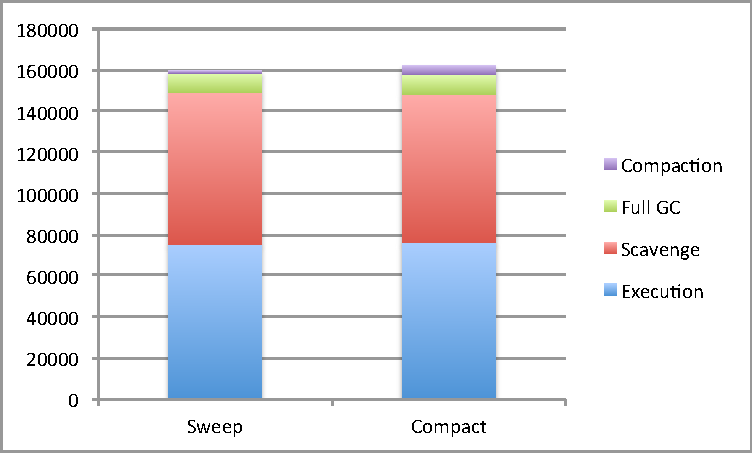
\includegraphics[width=\linewidth]{figures/load} 
	\subcaption{Load\vspace{0.5cm}}
   	\end{subfigure} \hspace{0.03\textwidth} \begin{subfigure}[b]{.48\textwidth}
	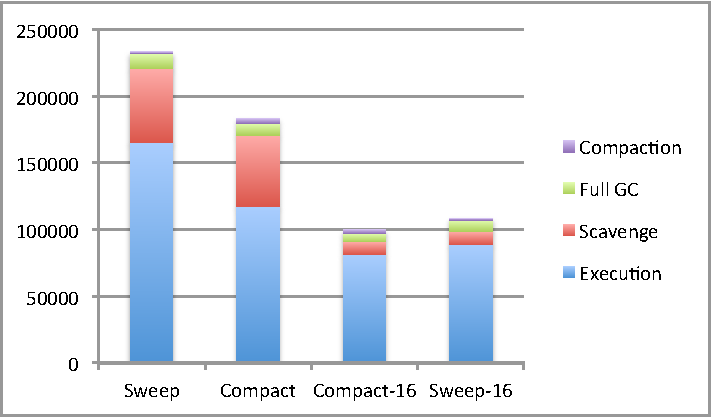
\includegraphics[width=\linewidth]{figures/prop} 
	\subcaption{ExpandProperties\vspace{0.5cm}}
   	\end{subfigure}
	
	\begin{subfigure}[b]{.48\textwidth}
	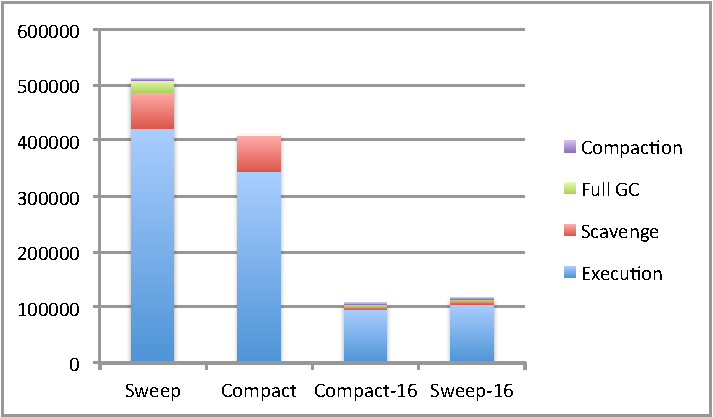
\includegraphics[width=\linewidth]{figures/propCache} 
	\subcaption{ExpandPropertiesWithCache}
   	\end{subfigure} \hspace{0.03\textwidth}  \begin{subfigure}[b]{.48\textwidth}
	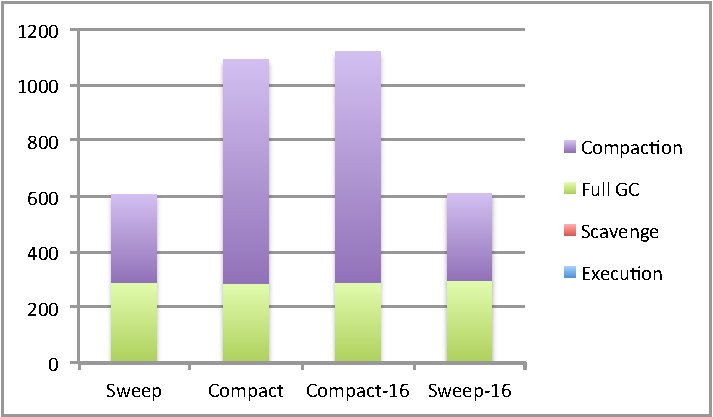
\includegraphics[width=\linewidth]{figures/release} 
	\subcaption{release}
   	\end{subfigure}
\caption{Moose benchmark results piled up.}
\label{MooseRes1}
\end{figure*}

\begin{figure*}[thb]
\begin{tabular}{|c|c|c|c|c|c|c|c|}
   \hline
  & & Total   & Scavenge  & Total Full  & Compaction  & Initial  & Final \\
 Benchmark & &  Exec. time &  time & GC time &  time &  Heap size & Heap size \\
  & &  (ms) &  (ms) & (ms) &  (ms) &  (Mb) &  (Mb) \\
   \hline
   \multirow{2}{*}{Load} & Sweep 	& 159821 $\pm$ 2218 &	73599 $\pm$ 1281 	& 10863 $\pm$ 726 	&1398 $\pm$ 091 	& 193 $\pm$ 0 	& 959 $\pm$ 9.69 \\
    				    & Compact 	& 162305 $\pm$ 2790 &	72150 $\pm$ 0782 	& 14091 $\pm$ 972 	&4661 $\pm$ 289 	& 193 $\pm$ 0 	& 909 $\pm$ 9.69 \\
   \hline
   \multirow{2}{*}{ExpandProperties} 	& Sweep 		& 232940 $\pm$ 01287 &	55497 $\pm$ 0238 	& 12240 $\pm$ 285 	&1178 $\pm$ 6.66 	& 959 $\pm$ 9.69 & 1888 $\pm$ 0 \\
    				    			& Compact 	& 183314 $\pm$ 13090 &	53165 $\pm$ 2343 	& 12496 $\pm$ 197 	&3775 $\pm$ 0108 	& 909 $\pm$ 9.69 & 1938 $\pm$ 0 \\
   \hline
   ExpandProperties 		& Sweep 		& 510013 $\pm$ 05812 &	64234 $\pm$ 0823 	& 23225 $\pm$ 100 	&2011 $\pm$ 10 	& 1888 $\pm$ 0 	& 1888 $\pm$ 0 \\
   WithCache  			& Compact 	& 408169 $\pm$ 20444 &	64492 $\pm$ 1234 	& 0 $\pm$ 0 		&0 $\pm$ 0 		& 1938 $\pm$ 0 		& 1938 $\pm$ 0 \\
   \hline
   \multirow{2}{*}{Release} 	& Sweep 		& 0606 $\pm$ 16 		&	0 $\pm$ 0 	& 0605 $\pm$ 16 	&316 $\pm$ 12 		& 1888 $\pm$ 0 	& 534 $\pm$ 58 \\
    				    		& Compact 	& 1092 $\pm$ 02 	&	0 $\pm$ 0 	& 1092 $\pm$ 01 		&806 $\pm$ 03 			& 1938 $\pm$ 0 		& 193 $\pm$ 00 \\
   \hline
\end{tabular} 
\caption{Moose benchmark results with standard errors.}
\label{MooseRes2}
\end{figure*}

We evaluated the Moose benchmarks using the reference Mark-Compact and Mark-Sweep algorithm and by analysing the wildfly code base\footnote{http://www.wildfly.org/}. The results are shown in Figure \ref{MooseRes1} and \ref{MooseRes2}. In the results, the compaction time includes the time spent in the compact phase in the Mark-Compact and in the sweep phase in the Mark-Sweep. Total full GC time is the total time spent in full GCs, including the compaction time. Scavenge time is the time spent in scavenges, \emph{i.e.,} garbage collection of young objects only. Total execution time is the total execution time, including scavenge and full GC time.

\paragraph{Load.} The Load benchmark grows the memory by 750 Mb with Sweep and by 700 Mb with Compact. Compaction time is smaller for the sweep algorithm, making the benchmark a little bit faster in the Mark-Sweep, which is to be expected since Sweep does not need to waste time updating pointers because objects are not moved in memory.

\paragraph{ExpandProperties.} The ExpandProperties benchmark grows the memory by around 1 Gb. Compaction time is a little bit better with the sweep algorithm as for the previous benchmark, but execution time is much worse. We believe this is due to worse locality of objects.

\paragraph{ExpandPropertiesWithCache.} The ExpandPropertiesWithCache benchmark does not increase the overall memory size. Since the compacting GC has compacted the heap before starting the benchmark, there is enough room to allocate the large objects (large objects are allocated directly in old space) required by the benchmark and there is no need for a full GC during the benchmark. However, with the sweep algorithm, there are multiple small available memory chunks which are not big enough to hold all the requested large objects, so a full GC is required. In addition, execution time is worse, as for the previous benchmark.

\paragraph{Release.} The Release benchmark releases all the graphs. With the compacting GC, memory goes back to its original size. With Sweep, multiple memory segments are left with a few live objects, forbidding the OS to reclaim those segments. Hence, the memory decreases drastically, but not to the original size. Compaction time is much faster with Sweep, but as we have discussed, for less efficiency.

\subsection{Sophie section}

\todo{Sophie}
It would be nice to evaluate both Sweeper and Planning on what we've just discussed.

I think we show exec time, full gc time, scavenge time, compaction time.

\section{Related and Future Work}

\paragraph{GC benchmark suite.}
Dacapo + see ref in Dacapo. \cite{DacapoBench}
\todo{Sophie}

\paragraph{ACDC-JS.}
ACDC-JS \cite{ACDCJS} is a configurable benchmarking tool designed to specifically measure and stress allocation and deallocation time in the JavaScript memory management model. 
It builds a heap model based on the behavior of real-time applications and aims at providing significant insights on the JavaScript memory management that cannnot be obtained from standard benchmarking suites. The value of specific heap options can be set by the user. 
Their study shows the negative impact of object liveness (time between allocation and last access, leading to the objects to be in different spaces in the heap) and deallocation delay on allocation time. It also stresses the trade-offs between memory consumption and allocation latency.

\paragraph{Future work: more benchmarks.}
need to add more benchmarks based on Dacapo ?

\paragraph{Future work: stress GC tests.}
stress cases from Configurable

\paragraph{Future work: more options.}
\sk{maybe? I will add options in the configurator soon. Should I mention it here?}

%% Bibliography
\bibliographystyle{alpha}
\bibliography{sista}


\end{document}
